\documentclass{article}
\usepackage[utf8]{inputenc}
\usepackage[none]{hyphenat}
\usepackage[a4paper, total={7in, 8.5in}]{geometry}
\usepackage{graphicx}
\usepackage{amsmath}
\usepackage{amssymb}
\usepackage{mathtools}
\usepackage{bbm}
\usepackage{amsthm}
\usepackage{mathdots}
\usepackage{fancyhdr}
\usepackage[parfill]{parskip}
\usepackage{tikz}
\usepackage{subcaption}
\usepackage{hyperref}
\usepackage{minted}
\theoremstyle{definition}
\newtheorem{theorem}{Theorem}
\newtheorem{definition}{Definition}
\newtheorem{example}{Example}
\newenvironment{theoremqed}
    {\begin{theorem}}
    {\hfill \qedsymbol \end{theorem}}
\newenvironment{definitionqed}
    {\begin{definition}}
    {\hfill \qedsymbol \end{definition}}
\newenvironment{exampleqed}
    {\begin{example}}
    {\hfill \qedsymbol \end{example}}

\renewcommand{\qedsymbol}{\(\blacksquare\)}
\newcommand{\X}{\mathbf{X}}
\renewcommand{\P}{\mathbb{P}}

\setlength{\parskip}{2mm}

\begin{document}

\begin{titlepage}
    \centering
    \vspace*{3cm}
    {\huge \bfseries Bayesian Network with Discrete Random Variables and its Python Implementation \par}
    \vspace{5cm}
    {\Large Yuwei (Johnny) Meng \par}
    \vspace{3cm}
    {\large Department of Statistical Sciences, University of Toronto}
    \vfill
\end{titlepage}

\tableofcontents

\pagebreak

\section{Preface \& Acknowledgements}

One day before class, I was talking with Jae and Liam, two other students in STA410, about coming up with a cool name for our Python packages, and I was like ``Oh man I hate coming up with names!'' I do think that cool package names are good, and I admire people coming up with names like \texttt{PyTorch} and \texttt{Beautiful Soup} (when I first learned to use \texttt{Beautiful Soup} I was very confused how this is an HTML parsing library). But yeah, coming up with names doesn't work for me. Just \texttt{BayesNetwork}, or \texttt{BayesianNetwork}. It's cool. It's straightforward. No need to ponder on why \texttt{Beautiful Soup} is for HTML.

Bayesian Network, a variational model for exact inference. The first time I familiarized with this concept was in CSC384, and I thought that this model seems very versatile and powerful. The exposure to the D-Separation, Variable Elimination, and Viterbi algorithms in this course kept my interest in this model. Upon finishing CSC384, I never thought that I would encounter this concept again in CSC412, presented in a more theoretical and mathematical way. What's more, for the third time I was taught Hidden Markov Model in STA410, and I just can't throw this concept out of my mind now. Well, it's something that interests me, so I quickly chose this model to do as my STA410 project.

Here I would like to express my sincere gratitude to Professor Alice Gao in CSC384 for introducing Bayesian Network to me in a very entertaining way, to Professor Denys Linkov/Murat Erdogdu in CSC412/STA414 for incorporating theories of this model into the course, and definitely to Professor Scott Schwartz in STA410 for providing this project opportunity to me to have this model implemented in Python.

\copyright \ Copyright 2025 Johnny Meng

\pagebreak

\section{Bayesian Network}

\subsection{Motivation}

Consider a set of random variables \(\X = (X_1, \cdots, X_n)\) where each \(X_i\in \{x_i, \neg x_i\}\) is binary. To specify the joint distribution of \(\X\), we need to list out all the possible combinations:
\begin{align*}
    &\P(x_1, x_2, \cdots, x_n); \\
    &\P(\neg x_1, x_2, \cdots, x_n); \\
    &\P(x_1, \neg x_2, \cdots, x_n); \\
    &\vdots
\end{align*}
For \(n\) random variables, the number of joint probabilities is \(2^n - 1\), which quickly becomes intractable as \(n\) grows large, requiring a more efficient framework for modeling joint probabilities. Bayesian Network, or Directed Acyclic Graphical Model (DAGM), is one such framework exploiting \textit{Theorem \ref{thm:chain_rule}} below.

\begin{theoremqed} \label{thm:chain_rule}
    \textbf{(Chain Rule of Probability)} Let \(X_1, \cdots, X_n\) be random variables. Then the joint probability can be expressed as
    \begin{align*}
        \P(X_1, \cdots, X_n) &= \P(X_1) \P(X_2, X_3, \cdots, X_n | X_1) \\
        &= \P(X_1) \P(X_2 | X_1) \P(X_3, \cdots, X_n | X_1, X_2) \\
        &= \cdots \\
        &= \P(X_1) \P(X_2 | X_1) \P(X_3 | X_1, X_2) \cdots \P(X_n | X_1, X_2, \cdots, X_{n-1}) \\
        &= \prod_{i=1}^n \P(X_i | X_1, X_2, \cdots, X_{i-1}).
    \end{align*}
\end{theoremqed}

Thus, if we have prior knowledge about the conditional independence relationships between the random variables we are modeling, then we can express the joint distribution in a more compact form, which motivates the use of Bayesian Networks.

\subsection{Introduction to Bayesian Network}

An example of Bayesian Network is shown in \textit{Figure \ref{fig:bayesian_network}} below.

\begin{figure}[htbp]
    \centering
    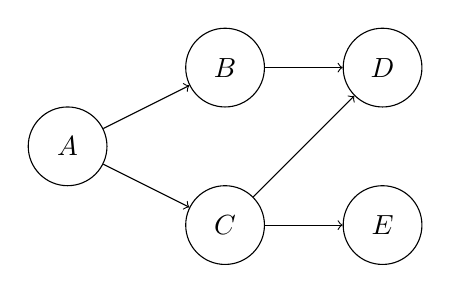
\begin{tikzpicture}
        \node[circle, draw, minimum size=1cm] (A) at (0,0) {\(A\)};
        \node[circle, draw, minimum size=1cm] (B) at (2,1) {\(B\)};
        \node[circle, draw, minimum size=1cm] (C) at (2,-1) {\(C\)};
        \node[circle, draw, minimum size=1cm] (D) at (4,1) {\(D\)};
        \node[circle, draw, minimum size=1cm] (E) at (4,-1) {\(E\)};

        \draw[->] (A) -- (B);
        \draw[->] (A) -- (C);
        \draw[->] (B) -- (D);
        \draw[->] (C) -- (D);
        \draw[->] (C) -- (E);
    \end{tikzpicture}
    \caption{Bayesian Network Example}
    \label{fig:bayesian_network}
\end{figure}

In this Bayesian Network, each vertex represents a random variable. The arrows denote conditional dependencies between random variables. For example, the edge \(A \longrightarrow B\) implies that \(B\) is directly conditionally dependent on \(A\). With this structure, we can model the joint distribution of these random variables in the following way:

\begin{definitionqed} \label{def:bayesian_network}
    Let \(\X = (X_1, \cdots, X_n)\) be a set of random variables modeled by a Bayesian Network. Then the joint probability can be expressed as
    \[\P(X_1, \cdots, X_n) = \prod_{i=1}^n \P(X_i | \operatorname{Parents}(X_i)).\]
\end{definitionqed}

\begin{exampleqed} \label{ex:bayesian_network}
    For the Bayesian Network shown in \textit{Figure \ref{fig:bayesian_network}}, the joint probability can be expressed as
    \[\P(A, B, C, D, E) = \P(A)\cdot\P(B|A)\cdot\P(C|A)\cdot\P(D|B,C)\cdot\P(E|C).\]
\end{exampleqed}

Note that \textit{Definition \ref{def:bayesian_network}} is a special case of \textit{Theorem \ref{thm:chain_rule}}, given that we have prior knowledge of the conditional independence relationships between the random variables. As a result, we can reduce the number of conditionals in the product and express the joint distribution in a more compact form. To illustrate this concept more clearly, let's define some probabilities for the Bayesian Network shown in \textit{Figure \ref{fig:bayesian_network}}. These probabilities will be used throughout the rest of this document.

\begin{exampleqed}
    Let \(A, B, C, D, E \in \{0, 1\}\) be binary random variables with the following conditional probabilities:

    \begin{figure}[htbp]
        \centering
        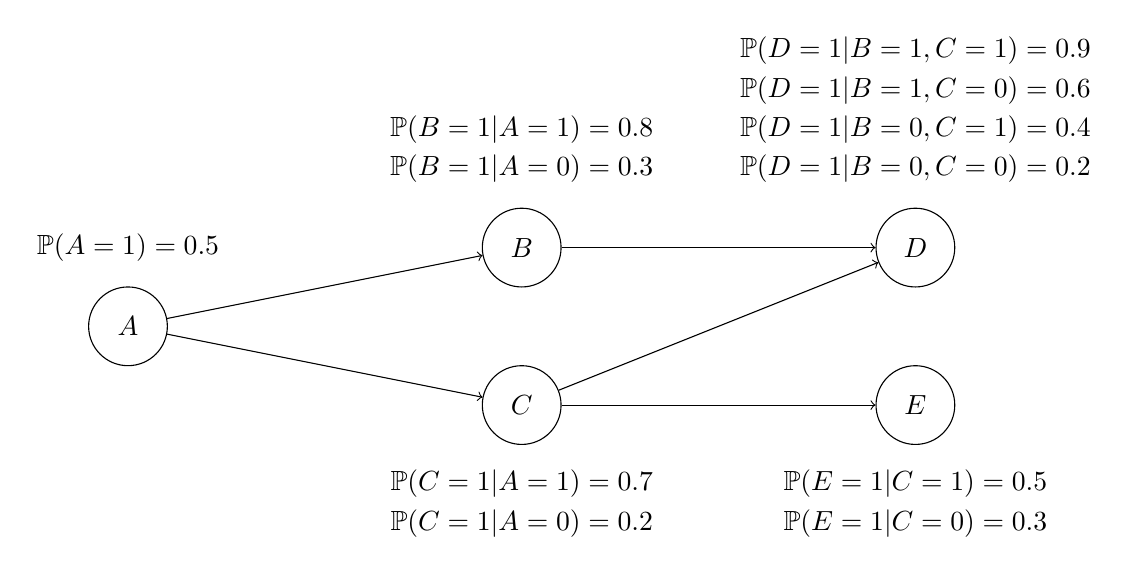
\begin{tikzpicture}
            \node[circle, draw, minimum size=1cm] (A) at (0,0) {\(A\)};
            \node[circle, draw, minimum size=1cm] (B) at (5,1) {\(B\)};
            \node[circle, draw, minimum size=1cm] (C) at (5,-1) {\(C\)};
            \node[circle, draw, minimum size=1cm] (D) at (10,1) {\(D\)};
            \node[circle, draw, minimum size=1cm] (E) at (10,-1) {\(E\)};
    
            \node (P_A) at (0,1) {\(\P(A=1)=0.5\)};
            \node (P_B_A1) at (5,2.5) {\(\P(B=1|A=1)=0.8\)};
            \node (P_B_A0) at (5,2) {\(\P(B=1|A=0)=0.3\)};
            \node (P_C_A1) at (5,-2) {\(\P(C=1|A=1)=0.7\)};
            \node (P_C_A0) at (5,-2.5) {\(\P(C=1|A=0)=0.2\)};
            \node (P_D_B1_C1) at (10,3.5) {\(\P(D=1|B=1,C=1)=0.9\)};
            \node (P_D_B1_C0) at (10,3) {\(\P(D=1|B=1,C=0)=0.6\)};
            \node (P_D_B0_C1) at (10,2.5) {\(\P(D=1|B=0,C=1)=0.4\)};
            \node (P_D_B0_C0) at (10,2) {\(\P(D=1|B=0,C=0)=0.2\)};
            \node (P_E_C1) at (10,-2) {\(\P(E=1|C=1)=0.5\)};
            \node (P_E_C0) at (10,-2.5) {\(\P(E=1|C=0)=0.3\)};
    
            \draw[->] (A) -- (B);
            \draw[->] (A) -- (C);
            \draw[->] (B) -- (D);
            \draw[->] (C) -- (D);
            \draw[->] (C) -- (E);
        \end{tikzpicture}
        \caption{Bayesian Network with Probabilities Example}
        \label{fig:bayesian_network_probs}
    \end{figure}
\end{exampleqed}

Note that only 11 conditional probabilities are needed to specify the joint distribution of the 5 random variables in our Bayesian Network, which is a significant improvement compared to the \(2^5 - 1 = 31\) joint probabilities in the general case. The exact number of required conditional probabilities depends on the structure of the Bayesian Network, though, but as long as there are some conditional independence relationships between the random variables, we can always expect a reduction in the number of required conditional probabilities.

\subsection{Implementation}

The implementation of Bayesian Network in this project consists of multiple modules which are discussed separately in the following subsections.

\subsubsection{\texttt{Distribution}}

The \texttt{distribution.py} file defines an abstract class called \texttt{Distribution}, as well as two inherited classes named \texttt{UnconditionalDistribution} and \texttt{ConditionalDistribution}. The purpose of these classes is to provide a data structure that encodes the probability distribution of a vertex in the Bayesian Network.

The abstract class \texttt{Distribution} has the attribute and method definitions:

\begin{minted}{python}
    domain: set
\end{minted}

This attribute defines the set of possible values for the random variables.

\begin{minted}{python}
    __call__(self, *args) -> float
\end{minted}

This method evaluates the probability of the random variable taking on a specific value in the domain.

\subsubsection{\texttt{UnconditionalDistribution}}

The \texttt{UnconditionalDistribution} class defines the distribution of a random variable that does not have a parent in the Bayesian Network, as well as the distribution of a random variable conditioned on its parents. Besides the inherited attribute \texttt{domain}, it has the following attribute:

\begin{minted}{python}
    distribution: dict[Any, float]
\end{minted}

This attribute serves as a lookup table for the unconditional distribution of the random variable. The keys of the dictionary are the possible values of the random variable, and the values are the corresponding probabilities.

\begin{minted}{python}
    __init__(self, domain: set, distribution: dict[Any, float]) -> None
\end{minted}

This is the constructor of the class. It takes in the domain and the distribution as arguments. The constructor checks if the provided domain and distribution are valid. If \texttt{domain} does not match the keys of \texttt{distribution}, or the probabilities in \texttt{distribution} do not sum to 1, a \texttt{ValueError} will be raised.

This class also implements the \texttt{\_\_call\_\_} method. The expected argument is a value in the domain of the random variable, and the method outputs the probability of the random variable taking on that value. If the argument is not in the domain, a \texttt{ValueError} will be raised.

\begin{exampleqed}
    For the Bayesian Network shown in \textit{Figure \ref{fig:bayesian_network_probs}}, the distribution of vertex \(A\) would have the following behaviors:

    \begin{minted}{python}
        >>> dist_A = UnconditionalDistribution(domain={0, 1}, distribution={0: 0.5, 1: 0.5})
        >>> dist_A(0)
        0.5
        >>> dist_A(1)
        0.5
    \end{minted}
\end{exampleqed}

\subsubsection{\texttt{ConditionalDistribution}}

This class defines the distribution of a random variable that has parents in the Bayesian Network. It inherits the \texttt{domain} attribute from the \texttt{Distribution} class, and it has the following attributes:

\begin{minted}{python}
    distributions[frozenset[str], UnconditionalDistribution]
\end{minted}

The keys of this dictionary are \texttt{frozenset}s of conditionals of the random variable, and the values define the distribution of the random variable conditioned on the values of its parents.

\begin{minted}{python}
    __init__(self,
             domain: set,
             distributions: dict[frozenset[str], UnconditionalDistribution]) -> None
\end{minted}

This constructor takes in the domain and the distributions as arguments. The constructor checks if the provided domain and distributions are valid. If \texttt{domain} does not match the domain of each \texttt{UnconditionalDistribution} object in \texttt{distribution}, a \texttt{ValueError} will be raised.

This class also implements the \texttt{\_\_call\_\_} method. The expected arguments are a value in the domain of the random variable and a dictionary of the values of its parents. The method outputs the probability of the random variable taking on that value, given the values of its parents. If the value is not in the domain, or if the parents are not in the dictionary, or if the conditioning values are not in the domain of the parents, a \texttt{ValueError} will be raised.

This is slightly confusing, so the following example illustrates this concept.

\begin{exampleqed}
    For the Bayesian Network shown in \textit{Figure \ref{fig:bayesian_network_probs}}, the distribution of vertex \(D\) would have the following behaviors:

    \begin{minted}{python}
        >>> dist_D_B1C1 = UnconditionalDistribution(domain={0, 1}, distribution={0: 0.1, 1: 0.9})
        >>> dist_D_B1C0 = UnconditionalDistribution(domain={0, 1}, distribution={0: 0.4, 1: 0.6})
        >>> dist_D_B0C1 = UnconditionalDistribution(domain={0, 1}, distribution={0: 0.6, 1: 0.4})
        >>> dist_D_B0C0 = UnconditionalDistribution(domain={0, 1}, distribution={0: 0.8, 1: 0.2})
        >>> dist_D = ConditionalDistribution(domain={0, 1}, distributions={
            frozenset({'B: 1', 'C: 1'}): dist_D_B1C1,
            frozenset({'B: 1', 'C: 0'}): dist_D_B1C0,
            frozenset({'B: 0', 'C: 1'}): dist_D_B0C1,
            frozenset({'B: 0', 'C: 0'}): dist_D_B0C0
        })
        >>> dist_D(1, {'B': 1, 'C': 0})
        0.6
        >>> dist_D(0, {'C': 0, 'B': 0})
        0.8
    \end{minted}
\end{exampleqed}

The use of a \texttt{frozenset} data structure is a compromise to the need for a hashable data structure. The advantage is that we don't need to memorize the order of the parents when we are looking up the distribution because there is no inherent order for a \texttt{set} object. When looking up probabilities, the order in which we pass in the parents thus does not matter, as long as the values are correct, which ensures the efficiency of the lookup process.

\subsubsection{\texttt{Vertex}}

The \texttt{Vertex} class represents a vertex in the Bayesian Network. It has the following attributes:

\begin{minted}{python}
    name: str
\end{minted}

This attribute defines the name of the vertex.

\begin{minted}{python}
    domain: set
\end{minted}

This attribute defines the set of possible values for the random variable.

\begin{minted}{python}
    parents: dict[str, Self]
    children: dict[str, Self]
\end{minted}

These two attributes hold the parents and children of the vertex in the Bayesian Network. The keys of the dictionaries are the names of the vertices, and the values are the corresponding \texttt{Vertex} objects.

\begin{minted}{python}
    distribution: Optional[Distribution]
\end{minted}

This attribute holds the distribution of the vertex. Depending on whether the vertex has parents or not, this attribute can be either an \texttt{UnconditionalDistribution} or a \texttt{ConditionalDistribution} object.

The \texttt{Vertex} class also implements the following methods:

\begin{minted}{python}
    __init__(self, name: str, domain: set) -> None
\end{minted}

This constructor takes in the name and domain of the vertex as arguments. It initializes the \texttt{parents}, \texttt{children}, and \texttt{distribution} attributes to empty dictionaries or \texttt{None}.

\begin{minted}{python}
    add_parent(self, parent: Self) -> None
    add_child(self, child: Self) -> None
\end{minted}

These two methods add a parent or child to the vertex. If the added vertex is already a parent or child of the vertex, a \texttt{ValueError} will be raised.

\begin{minted}{python}
    in_domain(self, value: Any) -> bool
\end{minted}

This method returns \texttt{True} if the value is in the domain of the vertex, and \texttt{False} otherwise.

\begin{minted}{python}
    set_distribution(self, distribution: Distribution) -> None
\end{minted}

This method sets the distribution of the vertex. This method contains many checks to ensure that \texttt{distribution} is valid. If \texttt{distribution} is not compatible with the vertex, a \texttt{ValueError} will be raised.

\begin{minted}{python}
    __call__(self, *args) -> float
\end{minted}

This method basically calls the \texttt{\_\_call\_\_} method of the \texttt{distribution} object with the arguments \texttt{*args}. The expected arguments are the same as the \texttt{\_\_call\_\_} method of the \texttt{distribution} object and outputs a probability. If the \texttt{distribution} attribute for the vertex is \texttt{None}, a \texttt{ValueError} will be raised.

\subsubsection{\texttt{BayesNetwork}}

This class represents the Bayesian Network. It has the following attribute:

\begin{minted}{python}
    vertices: dict[str, Vertex]
\end{minted}

This attribute holds a list of the vertices in the Bayesian Network. The keys of the dictionary are the names of the vertices, and the values are the corresponding \texttt{Vertex} objects.

The \texttt{BayesNetwork} class implements the following methods:

\begin{minted}{python}
    __init__(self) -> None
\end{minted}

The constructor creates a \texttt{BayesNetwork} object and initializes the \texttt{vertices} attribute to an empty dictionary.

\begin{minted}{python}
    __len__(self) -> int
\end{minted}

This method returns the number of vertices in the Bayesian Network.

\begin{minted}{python}
    add_node(self, vertex: Vertex) -> None
\end{minted}

This method adds a vertex to the Bayesian Network. If the vertex is already in the network, a \texttt{ValueError} will be raised.

\begin{minted}{python}
    add_edge(self, parent: Vertex, child: Vertex) -> None
\end{minted}

This method adds an edge from the parent vertex to the child vertex in the Bayesian Network. If either vertex is not in the network, a \texttt{ValueError} will be raised.

\begin{minted}{python}
    find_roots(self) -> list[Vertex]
\end{minted}

This method returns a list of the root vertices in the Bayesian Network. A root vertex is defined as a vertex that does not have any parents in the network.

\begin{minted}{python}
    __call__(self, *args) -> float
\end{minted}

This method evaluates the joint probability of the random variables in the Bayesian Network. The expected argument is a dictionary with the keys being the names of the random variables and the values being the corresponding values. The method outputs the joint probability of the random variables taking on those values. If values for one or more random variables are not provided, a \texttt{ValueError} will be raised. To compute the probability of a subset of the random variables, use the \textit{Variable Elimination} algorithm discussed in the next section.

\subsubsection{\texttt{read\_bayes\_network\_from\_txt}}

The above description might be very confusing, so it is not recommended to create a Bayesian Network from scratch. Instead, I provide a function to read in a Bayesian Network from a text file. An example of this text file is provided in this \href{https://github.com/BullDF/bayes_network/blob/main/bn_ex.txt}{\texttt{bn\_ex.txt}} file. The text file requires 3 parts, explained using the example file and \textit{Figure \ref{fig:bayesian_network_probs}}:

\begin{verbatim}
    A: {0, 1}
    B: {0, 1}
    C: {0, 1}
    D: {0, 1}
    E: {0, 1}
\end{verbatim}

This part defines the vertices in the Bayesian Network. Each line contains the name of the vertex and its domain, enclosed in curly braces. The vertices are separated by new lines.

\begin{verbatim}
    A -> B
    A -> C
    B -> D
    C -> D
    C -> E
\end{verbatim}

This part defines the edges in the Bayesian Network. Each line contains the name of the parent vertex and the name of the child vertex, separated by an arrow (\texttt{->}). The edges are separated by new lines.

\begin{verbatim}
    P(A = 1) = 0.5
    P(A = 0) = 0.5

    P(B = 1 | A = 1) = 0.8
    P(B = 0 | A = 1) = 0.2
    P(B = 1 | A = 0) = 0.3
    P(B = 0 | A = 0) = 0.7

    P(D = 1 | B = 1, C = 1) = 0.9
    P(D = 0 | B = 1, C = 1) = 0.1
    P(D = 1 | B = 1, C = 0) = 0.6
    P(D = 0 | B = 1, C = 0) = 0.4
    P(D = 1 | B = 0, C = 1) = 0.4
    P(D = 0 | B = 0, C = 1) = 0.6
    P(D = 1 | B = 0, C = 0) = 0.2
    P(D = 0 | B = 0, C = 0) = 0.8
    
    ...
\end{verbatim}

This part defines the unconditional and conditional distributions of the vertices in the Bayesian Network. The conditional distributions are separated by new lines. Note that it is necessary to provide the probabilities for both \texttt{P(A = 1)} and \texttt{P(A = 0)} in the text file, even though the complement can be easily computed.

As long as the format is followed, the order in which the vertices, edges, and distributions are defined does not matter because the function uses regular expression to parse the text file. The function will create a \texttt{BayesNetwork} object and add the vertices, edges, and distributions to the object. The function then returns the \texttt{BayesNetwork} object. It is strongly recommended to use this function to create a Bayesian Network.

To wrap up this section, below is an example of how to use the function to create a Bayesian Network from a text file.

\begin{exampleqed}
    Assume that the text file is named \texttt{\texttt{bn\_ex.txt}} and is in the same directory as the Python file.

    \begin{minted}{python}
        >>> bn = read_bayes_network_from_txt('bn_ex.txt')
        >>> bn.find_roots()
        [A: {0, 1}]
        >>> len(bn)
        5
    \end{minted}

    Regarding joint probability computations:
    \begin{align*}
        \P(A=1, B=0, C=1, D=1, E=0) &= \P(A=1)\P(B=0|A=1)\P(C=1|A=1)\P(D=1|B=0,C=1) \\
        &\cdot \P(E=0|C=1) \\
        &= 0.5 \cdot 0.2 \cdot 0.7 \cdot 0.4 \cdot 0.5 \\
        &= 0.014.
    \end{align*}

    The code output confirms this result:

    \begin{minted}{python}
        >>> bn({'A': 1, 'B': 0, 'C': 1, 'D': 1, 'E': 0})
        0.013999999999999999 # Numerical roundoff error
    \end{minted}
\end{exampleqed}

\pagebreak

\section{Variable Elimination}

\subsection{Motivation}

In the previous section, we introduced how we could easily compute the joint probability of the random variables in a Bayesian Network. However, \textit{Definition \ref{def:bayesian_network}} must be used when the joint probability involves all random variables in the network and cannot be applied when we want to calculate the joint probability of a subset of the random variables or a conditional probability of the random variables. This motivates the use of the Variable Elimination algorithm.

Below is the example Bayesian Network again for reference:
\begin{figure}[htbp]
    \centering
    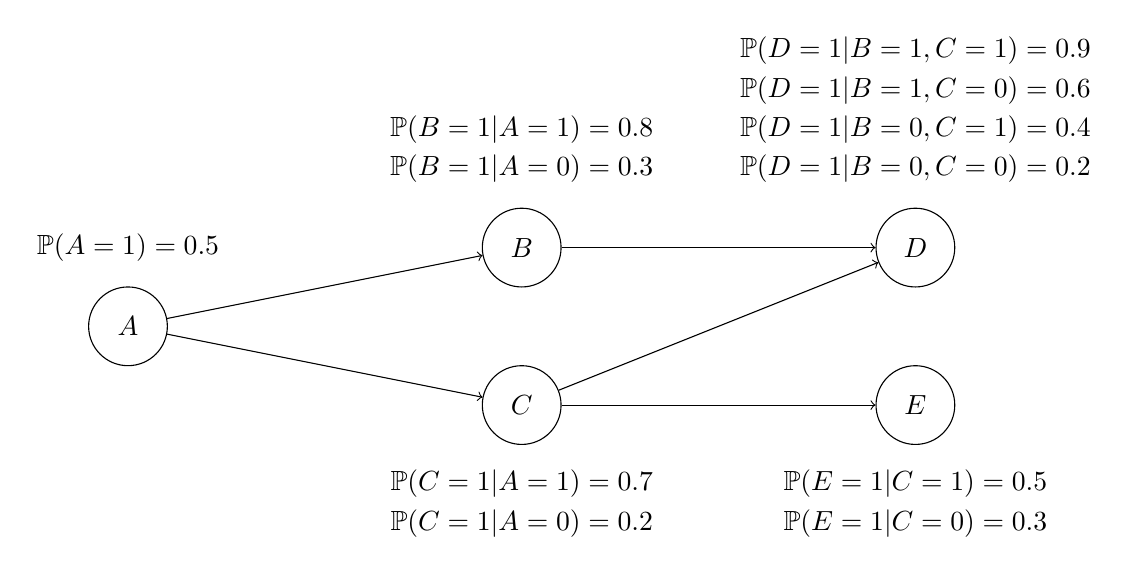
\begin{tikzpicture}
        \node[circle, draw, minimum size=1cm] (A) at (0,0) {\(A\)};
        \node[circle, draw, minimum size=1cm] (B) at (5,1) {\(B\)};
        \node[circle, draw, minimum size=1cm] (C) at (5,-1) {\(C\)};
        \node[circle, draw, minimum size=1cm] (D) at (10,1) {\(D\)};
        \node[circle, draw, minimum size=1cm] (E) at (10,-1) {\(E\)};

        \node (P_A) at (0,1) {\(\P(A=1)=0.5\)};
        \node (P_B_A1) at (5,2.5) {\(\P(B=1|A=1)=0.8\)};
        \node (P_B_A0) at (5,2) {\(\P(B=1|A=0)=0.3\)};
        \node (P_C_A1) at (5,-2) {\(\P(C=1|A=1)=0.7\)};
        \node (P_C_A0) at (5,-2.5) {\(\P(C=1|A=0)=0.2\)};
        \node (P_D_B1_C1) at (10,3.5) {\(\P(D=1|B=1,C=1)=0.9\)};
        \node (P_D_B1_C0) at (10,3) {\(\P(D=1|B=1,C=0)=0.6\)};
        \node (P_D_B0_C1) at (10,2.5) {\(\P(D=1|B=0,C=1)=0.4\)};
        \node (P_D_B0_C0) at (10,2) {\(\P(D=1|B=0,C=0)=0.2\)};
        \node (P_E_C1) at (10,-2) {\(\P(E=1|C=1)=0.5\)};
        \node (P_E_C0) at (10,-2.5) {\(\P(E=1|C=0)=0.3\)};

        \draw[->] (A) -- (B);
        \draw[->] (A) -- (C);
        \draw[->] (B) -- (D);
        \draw[->] (C) -- (D);
        \draw[->] (C) -- (E);
    \end{tikzpicture}
    \caption{Bayesian Network with Probabilities Example}
    \label{fig:bayesian_network_probs_ch3}
\end{figure}

Some examples of probabilities we might want to compute are as follows:
\begin{align*}
    &\P(A, B, C, D); \\
    &\P(B, C | D); \\
    &\P(B, E | A); \\
    &\P(A, B | C, D); \\
    &\P(E); \\
    &\vdots
\end{align*}

With the Variable Elimination algorithm, these probabilities can be computed easily.

\subsection{Theory}

The Variable Elimination algorithm is based on the following theorem:

\begin{theoremqed} \label{thm:marginal}
    Given discrete random variables \(X, Y\), the marginal probabilities can be computed as
    \begin{align*}
        p_X(x) &= \sum_y p_{XY}(x, y) \\
        &= \sum_y p_{X|Y}(x|y) p_Y(y); \\
        p_Y(y) &= \sum_x p_{XY}(x, y) \\
        &= \sum_x p_{Y|X}(y|x) p_X(x).
    \end{align*}
\end{theoremqed}

With \textit{Theorem \ref{thm:marginal}}, the Variable Elimination algorithm is as follows:

\begin{theoremqed} \label{thm:vea}
    \textbf{(Variable Elimination Algorithm)} Given a Bayesian Network with vertices \(\X = \{X_1, \cdots, X_n\}\) and a desired probability \(\P(Q | E)\) with \(Q \subseteq \X\), \(E \subseteq \X\), \(Q \cap E = \varnothing\), define \(H = \X \setminus Q \cup E\) as the hidden variables. Let \(D_X\) denote the domain of random variable \(X\). Then
    \[\P(Q | E) = \operatorname{normalize}\left(\sum_{X_h \in H} \sum_{x\in D_{X_h}} \prod_{\psi \in \mathcal{F}} \psi(X_h|E) \right),\]
    where the notation \(\psi(X_h|E)\) denotes the ``factor'' that concerns the hidden variable \(X_h\) conditioned on \(E\), and \(\mathcal{F}\) defines the set of all the ``factors''.
\end{theoremqed}

\textit{Theorem \ref{thm:vea}} defines some new concepts such as \textit{hidden variables} and \textit{factors} that might be confusing, so I devote the following section to give an example of using the Variable Elimination algorithm to compute a probability.

\subsection{Example}

Given Bayesian Network \textit{Figure \ref{fig:bayesian_network_probs_ch3}}, suppose we want to compute conditional probability
\[\P(A, E | D = 0).\]

\subsubsection{Step I -- Creating Initial Factors}

For each node in the Bayesian Network, we create a factor consisting of its probabilities defined by the network. Each factor has a scope denoting the set of random variables it concerns. For the Bayesian Network in \textit{Figure \ref{fig:bayesian_network_probs_ch3}}, we would create the following initial factors:
\begin{align*}
    f_1(A) &= \begin{pmatrix}
        A = 1 & 0.5 \\
        A = 0 & 0.5
    \end{pmatrix} \\
    f_2(A, B) &= \begin{pmatrix}
        A = 1 & B = 1 & 0.8 \\
        A = 1 & B = 0 & 0.2 \\
        A = 0 & B = 1 & 0.3 \\
        A = 0 & B = 0 & 0.7
    \end{pmatrix} \\
    f_3(A, C) &= \begin{pmatrix}
        A = 1 & C = 1 & 0.7 \\
        A = 1 & C = 0 & 0.3 \\
        A = 0 & C = 1 & 0.2 \\
        A = 0 & C = 0 & 0.8
    \end{pmatrix}
    \intertext{}
    f_4(B, C, D) &= \begin{pmatrix}
        B = 1 & C = 1 & D = 1 & 0.9 \\
        B = 1 & C = 1 & D = 0 & 0.1 \\
        B = 1 & C = 0 & D = 1 & 0.6 \\
        B = 1 & C = 0 & D = 0 & 0.4 \\
        B = 0 & C = 1 & D = 1 & 0.4 \\
        B = 0 & C = 1 & D = 0 & 0.6 \\
        B = 0 & C = 0 & D = 1 & 0.2 \\
        B = 0 & C = 0 & D = 0 & 0.8
    \end{pmatrix} \\
    f_5(C, E) &= \begin{pmatrix}
        C = 1 & E = 1 & 0.5 \\
        C = 1 & E = 0 & 0.5 \\
        C = 0 & E = 1 & 0.3 \\
        C = 0 & E = 0 & 0.7
    \end{pmatrix}
\end{align*}

Note that whether the probabilities are conditional or not do not matter in the factors. The factors only care about the random variables they concern. As a reference, the set of factors we have after step 1 is
\[\mathcal{F}_1 = \{f_1, f_2, f_3, f_4, f_5\}.\]

\subsubsection{Step II -- Restricting Evidence}

The evidence we have is \(D = 0\), and so we can discard entries of \(D\) that are irrelevant. Specifically, \(f_4\) turns into
\[f_6(B, C) = \begin{pmatrix}
    B = 1 & C = 1 & 0.1 \\
    B = 1 & C = 0 & 0.4 \\
    B = 0 & C = 1 & 0.6 \\
    B = 0 & C = 0 & 0.8
\end{pmatrix}\]
Note that we can also remove \(D\) from the scope of \(f_4\) because we have restricted it based on the evidence.

After step 2, the set of factors is
\[\mathcal{F}_2 = \{f_1, f_2, f_3, f_5, f_6\}.\]
Note that each factor is used only once and we can safely discard it afterwards.

\subsubsection{Step III -- Eliminating Hidden Variables}

In our probability, \(A, E\) are the \textit{Query} variables because we are interested in their joint probabilities. \(D\) is the \textit{Evidence} variable because we have evidence of it. The remaining variables, \(B\) and \(C\), are \textit{Hidden} variables, and we will be removing them in this step.

The computational complexity of the Variable Elimination algorithm is \(O(mk^{N_{\max}})\), where \(m\) is the number of initial factors, \(k\) is the maximum number of values in the domain of the variables, and \(N_{\max}\) is the number of variables inside the largest sum. However, this complexity largely depends on the order in which we eliminate the hidden variables, and finding the optimal order of elimination is \textsf{NP}-hard. For a small Bayesian Network like the one in our case, the order doesn't matter much, so I will predetermine the order to be \(B \to C\).

To eliminate \(B\), we will gather all factors that concern the variable \(B\), in our case they are \(f_2\) and \(f_6\). We will consider every valid combination of the variables and multiply the probability values if the conditions match. After multiplying, we get
\[f_7(A, B, C) = \begin{pmatrix}
    A = 1 & B = 1 & C = 1 & 0.8\cdot 0.1 = 0.08 \\
    A = 1 & B = 1 & C = 0 & 0.8\cdot 0.4 = 0.32 \\
    A = 1 & B = 0 & C = 1 & 0.2\cdot 0.6 = 0.12 \\
    A = 1 & B = 0 & C = 0 & 0.2\cdot 0.8 = 0.16 \\
    A = 0 & B = 1 & C = 1 & 0.3\cdot 0.1 = 0.03 \\
    A = 0 & B = 1 & C = 0 & 0.3\cdot 0.4 = 0.12 \\
    A = 0 & B = 0 & C = 1 & 0.7\cdot 0.6 = 0.42 \\
    A = 0 & B = 0 & C = 0 & 0.7\cdot 0.8 = 0.56
\end{pmatrix}\]
Next, we will sum out \(B\) and obtain
\[f_8(A, C) = \begin{pmatrix}
    A = 1 & C = 1 & 0.08 + 0.12 = 0.2 \\
    A = 1 & C = 0 & 0.32 + 0.16 = 0.48 \\
    A = 0 & C = 1 & 0.03 + 0.42 = 0.45 \\
    A = 0 & C = 0 & 0.12 + 0.56 = 0.68
\end{pmatrix}\]
Now we have eliminated variable \(B\). As a reference, the set of factors we have after this step is
\[\mathcal{F}_3 = \{f_1, f_3, f_5, f_8\}.\]
We will do the same thing for variable \(C\). We gather factors \(f_3\), \(f_5\) and \(f_8\) that concern \(C\), and we multiply them together:
\[f_9(A, C, E) = \begin{pmatrix}
    A = 1 & C = 1 & E = 1 & 0.7\cdot 0.5 \cdot 0.2 = 0.07 \\
    A = 1 & C = 1 & E = 0 & 0.7\cdot 0.5 \cdot 0.2 = 0.07 \\
    A = 1 & C = 0 & E = 1 & 0.3\cdot 0.3 \cdot 0.48 = 0.0432 \\
    A = 1 & C = 0 & E = 0 & 0.3\cdot 0.7 \cdot 0.48 = 0.1008 \\
    A = 0 & C = 1 & E = 1 & 0.2\cdot 0.5 \cdot 0.45 = 0.045 \\
    A = 0 & C = 1 & E = 0 & 0.2\cdot 0.5 \cdot 0.45 = 0.045 \\
    A = 0 & C = 0 & E = 1 & 0.8\cdot 0.3 \cdot 0.68 = 0.1632 \\
    A = 0 & C = 0 & E = 0 & 0.8\cdot 0.7 \cdot 0.68 = 0.3808
\end{pmatrix}\]
Then, we sum out \(C\):
\[f_{10}(A, E) = \begin{pmatrix}
    A = 1 & E = 1 & 0.07 + 0.0432 = 0.1132 \\
    A = 1 & E = 0 & 0.07 + 0.1008 = 0.1708 \\
    A = 0 & E = 1 & 0.045 + 0.1632 = 0.2082 \\
    A = 0 & E = 0 & 0.045 + 0.3808 = 0.4258
\end{pmatrix}\]
After this step, the remaining factors are
\[\mathcal{F}_4 = \{f_1, f_{10}\}.\]

\subsubsection{Step IV -- Combining and Normalization}

At this step, all remaining factors should concern only our query variables. We will combine the remaining factors (\(f_1, f_{10}\)) by multiplying them like we did previously:
\[f_{11}(A, E) = \begin{pmatrix}
    A = 1 & E = 1 & 0.5\cdot 0.1132 = 0.0566 \\
    A = 1 & E = 0 & 0.5\cdot 0.1708 = 0.0854 \\
    A = 0 & E = 1 & 0.5\cdot 0.2082 = 0.1041 \\
    A = 0 & E = 0 & 0.5\cdot 0.4258 = 0.2129
\end{pmatrix}\]

We are almost done. We just need to normalize the remaining values so that they follow a probability distribution. The current sum is \(0.0566 + 0.0854 + 0.1041 + 0.2129 = 0.459\). We can normalize the values by dividing each value by the sum, rounded to 3 decimal points:
\[\P(A, E | D = 0) = \begin{pmatrix}
    A = 1 & E = 1 & 0.0566/0.459 = 0.123 \\
    A = 1 & E = 0 & 0.0854/0.459 = 0.186 \\
    A = 0 & E = 1 & 0.1041/0.459 = 0.227 \\
    A = 0 & E = 0 & 0.2129/0.459 = 0.464
\end{pmatrix}\]

\subsection{Implementation}

The Variable Elimination algorithm is implemented in the \texttt{variable\_elimination.py} file. Each step mentioned above gets its own helper function, but the entire pipeline can be executed by calling the \texttt{variable\_elimination} function. This function has the following signature:

\begin{minted}{python}
    variable_elimination(bn: BayesNetwork, query: set, evidence: dict={}) -> dict
\end{minted}

Running code for the example illustrated above, we would get the outputs

\begin{minted}{python}
    >>> bn = read_bayes_network_from_txt('bn_ex.txt')
    >>> variable_elimination(bn, query={'A', 'E'}, evidence={'D': 0})
    {{'A: 1', 'E: 1'}: 0.12331154684095862,
     {'E: 1', 'A: 0'}: 0.22679738562091506,
     {'A: 1', 'E: 0'}: 0.18605664488017432,
     {'E: 0', 'A: 0'}: 0.46383442265795205}
\end{minted}

which match our manual calculations above.

\pagebreak

\section{Hidden Markov Model}

\pagebreak

\section{The Viterbi Algorithm}

\pagebreak

\section{The Forward-Backward Algorithm}

\end{document}